\chapter{Kravspecifikation} \label{ch:kravspecifikation}
\section*{Version}
\begin{table}[h]
	\centering
	\begin{tabularx}{\textwidth - 2cm}{|l|l|l|X|}
	\hline
	Dato			& Version			& Initialer 		& Ændring										\\ \hline
	29. september 	& 1 				& Alle				& Første udkast. 								\\ \hline
	26. oktober		& 2 				& PKP, KT og JEP	& Mindre rettelser efter review						 						\\ \hline
			 		& 3 				&  					& 												\\ \hline
					& 4 				&  					& 												\\ \hline
	\end{tabularx}
\end{table}
\clearpage

%---------------------------------------------------------------------------------------
%											SYSTEMOVERSIGT
%---------------------------------------------------------------------------------------


\section{Systemoversigt} \label{sec:systemoversigt}
På figur \ref{fig:systemoversigt} ses den overordnede systemoversigt med kommunikationsveje og mekaniske forbindelser. Diagrammet skal give læseren et hurtigt overblik over det samlede system. I afsnittet %TODO henvisning
beskrives blokke og kommunikationsveje mere detaljeret. Under figur \ref{fig:systemoversigt} er blokkene kort beskrevet. 

\begin{figure}[h]
\centering
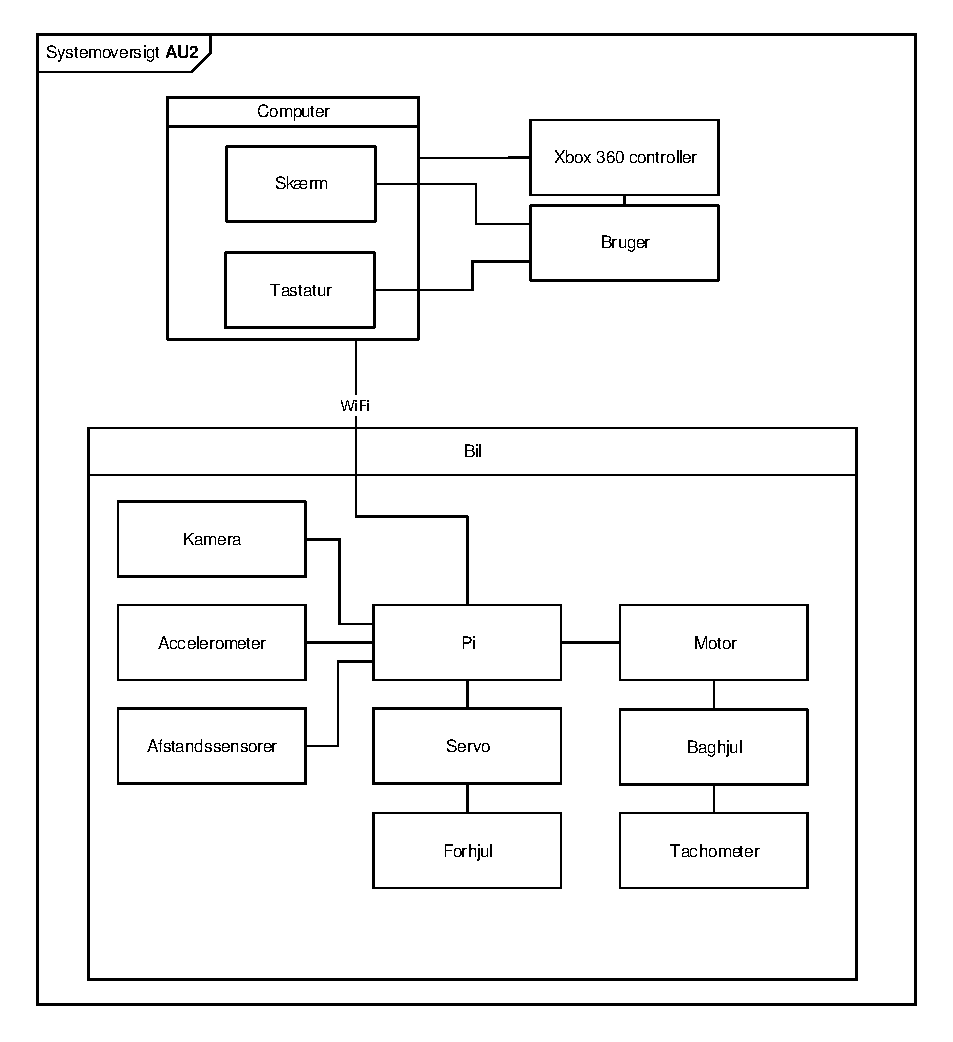
\includegraphics[width=\textwidth]{../fig/diagrammer/systemoversigt.pdf}
\caption{Overordnet systemoversigt}
\label{fig:systemoversigt}
\end{figure}
\clearpage

\subsubsection{Pi}
Systemets kerne er et Raspberry Pi 2 board.
Pi'en står for at processere data fra afstandsensorene, og håndtere streaming af video. Derudover afvikles regulering til motor, samt styring af servo også fra Pi'en. 

\subsubsection{Servomotor}
Servomotor har til opgave at omsætte signal fra Pi'en til mekanisk styring af bilens forhjul. 

\subsubsection{Afstandssensor}
Bilens 2 fremadrettet og 2 bagudrettet afstandssensorer har til formål at indsamle data om eventuelle forhindringer i bilen kørebane. 

\subsubsection{Accelerometer}
Der er påmonteret et accelerometer der anvendes til regulering af hastighed.

\subsubsection{Kamera}
Bilens kamera streamer video til PC'ens skærm så Bruger har mulighed for at navigere på baggrund af visuel feedback

\subsubsection{PC}
PC afvikler den software hvorigennem bilen kontrolleres, konfigureres og kalibreres. Det er ligeledes via computeren at Bruger får visuel feedback fra bilens kamera. 

\subsubsection{Xbox-360 Controller}
Til at kontrollere bilen, benyttes en Xbox-360 controller. vha. en række trykknapper og styrepinde kan bilens hastighed, såvel som retning bestemmes. 

\subsubsection{Motor}
Motoren omsætter data, herunder regulering fra Pi'en til mekanisk styring af bilens hastighed.

\subsubsection{Tachometer}
Motorens omdrejningshastighed kan via tachometeret aflæses og herefter benyttes til databehandling og regulering. 
\clearpage

I figur \ref{fig:main_menu} vises en skitse af hovedmenuen i softwaren på PC. 

\begin{figure}[h]
\centering
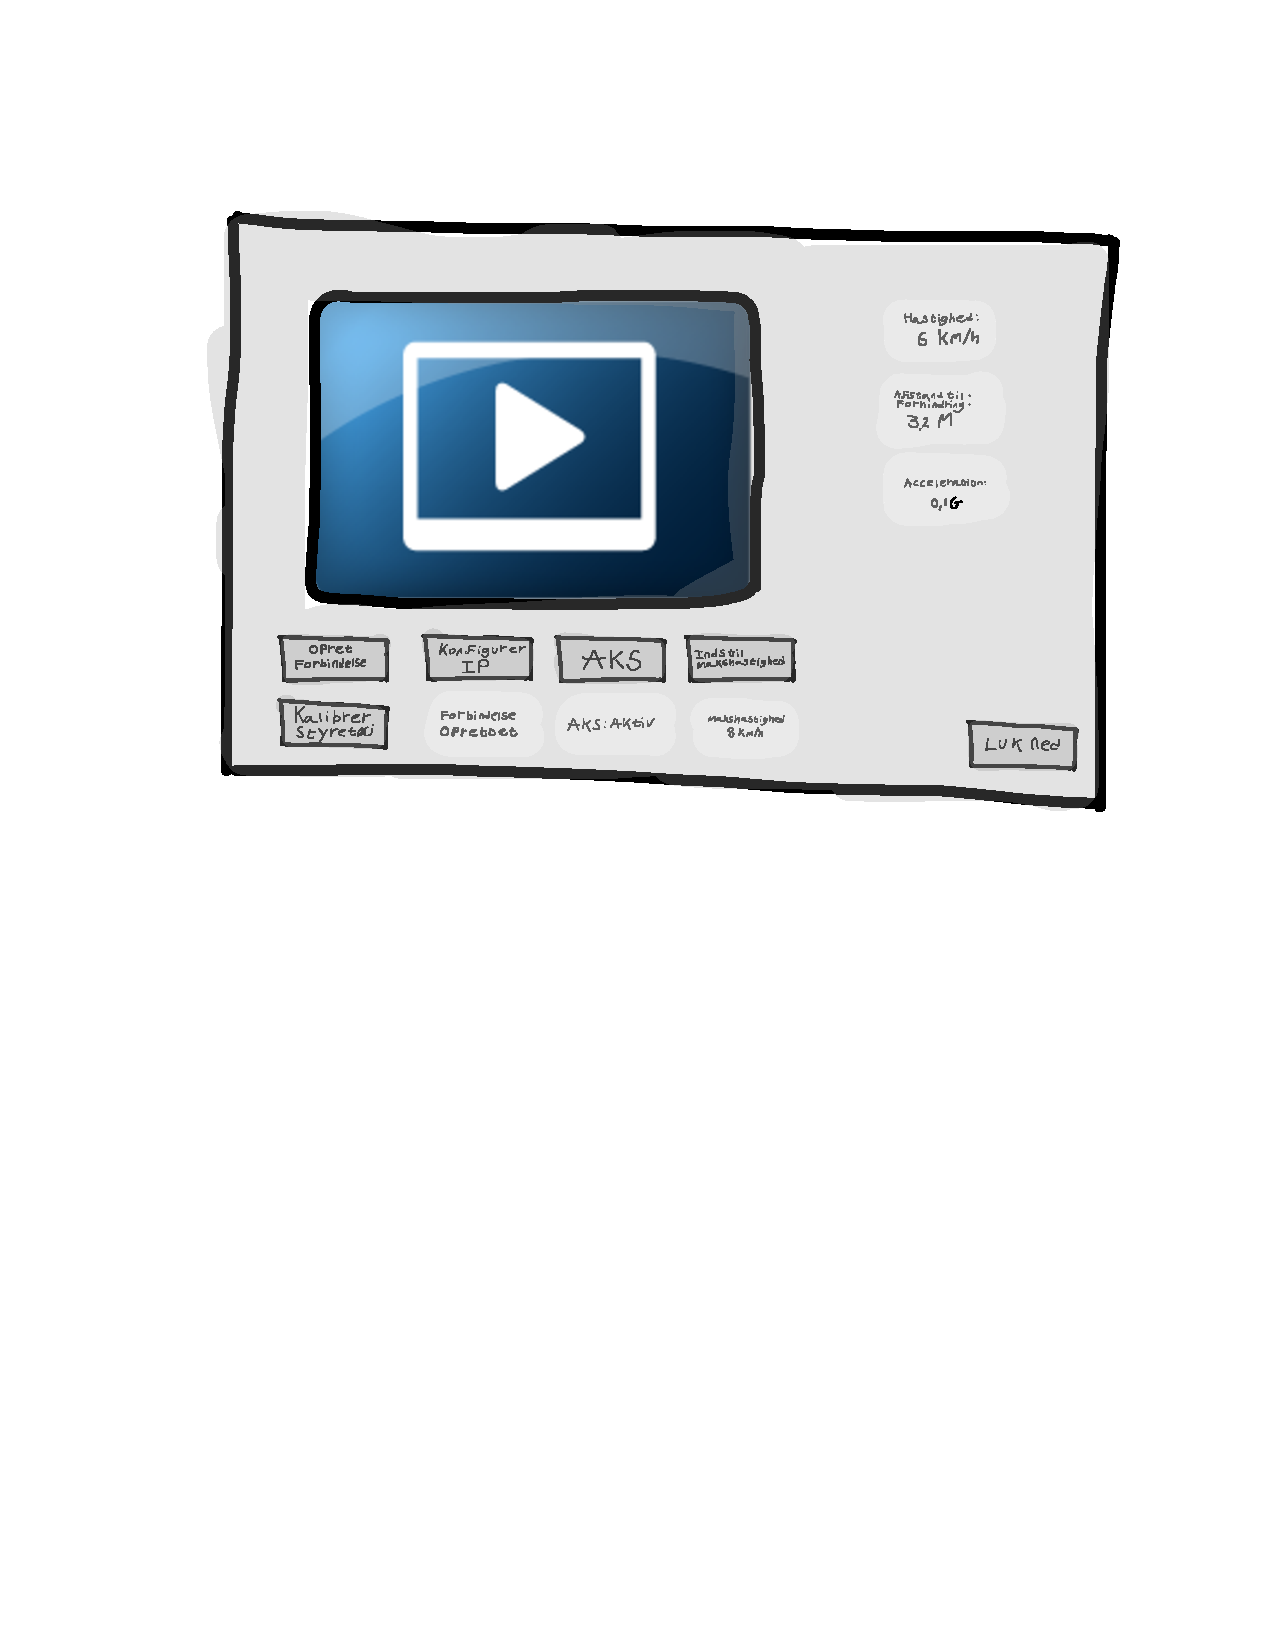
\includegraphics[width=\textwidth*2/3]{../fig/gui/hovedmenu}
\caption{Skitse af hovedmenu}
\label{fig:main_menu}
\end{figure}

\clearpage 
%---------------------------------------------------------------------------------------
%											AKTØR-KONTEKSTDIAGRAM
%---------------------------------------------------------------------------------------

\section{Aktør-kontekstdiagram} \label{sec:aktor-kontekstdiagram}
På figur \ref{fig:aktor_kontekst} ses aktørkontekstdiagram over systemet. 

\begin{figure}[h]
\centering
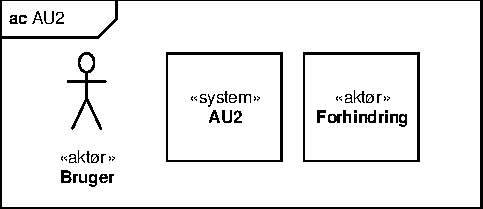
\includegraphics[scale=1.1]{../fig/diagrammer/ac_au2.pdf}
\caption{Aktør kontekst diagram for AU2.}
\label{fig:aktor_kontekst}
\end{figure}

%---------------------------------------------------------------------------------------
%											AKTØRBESKRIVELSER
%---------------------------------------------------------------------------------------

\section{Aktørbeskrivelser} \label{sec:aktorbeskrivelser}
Som figur \ref{fig:aktor_kontekst} viser, er der 2 aktører til systemet.
\textit{Bruger} og \textit{Forhindring}.

\subsubsection{Bruger - Primær Aktør}
Brugeren vil typisk være et barn med alder over 8 år, men kan også være en voksen med interesse for fjernstyrede biler.
\\ %TODO Indsæt linjeskift
Bruger kan:
\begin{itemize}
	\item Starte og stoppe systemet 
	\item Styre bilen over et Wi-Fi netværk.
	\item Konfigure og kalibrere system.
\end{itemize}

\subsubsection{Forhindring - Sekundær Aktør}
\textit{Forhindring} er objekter i det miljø bilen kører i, og som der dermed er risiko for at bilen kan kollidere med.  
\clearpage


\clearpage
%---------------------------------------------------------------------------------------
%									FUNKTIONELLE KRAV
%---------------------------------------------------------------------------------------

\section{Funktionelle krav} \label{sec:funktionelle_krav}
Ambitionen for dette projekt er som absolut minimum at realisere nedenstående punkter under \textit{''skal''}. 
Det forventes desuden at punkterne under \textit{''bør''} realiseres, men de har lavere prioritet.
Punkterne under \textit{''kan''} forventes ikke realiseret, og punkterne under \textit{''vil ikke...''} realiseres med sikkerhed ikke. 
Sidstnævnte punkter kan ses som udviklingsmuligheder i forhold til senere versioner af systemet. 

Systemet\ldots
\begin{enumerate}\itemsep1pt \parskip0pt \parsep0pt
	\item \ldots  \emph{Skal} kunne køre frem og tilbage.
	\item \ldots  \emph{Skal} kunne dreje.
	\item \ldots  \emph{Skal} kunne regulere hastigheden på bilen.
	\item \ldots  \emph{Skal} give Bruger mulighed for at begrænse maksimumshastighed.
	\item \ldots  \emph{Skal} give Bruger mulighed for manuel styring via Xbox-360 controller af hastighed og retning.
	\item \ldots  \emph{Skal} via Wi-Fi netværk kunne kommunikere mellem bil og PC.
	\item \ldots  \emph{Skal} kunne identificere forhindringer foran og bag bilen.
	\item \ldots  \emph{Skal} indeholde et anti-kollisionssystem baseret på afstandssensorer.
	\item \ldots  \emph{Skal} via. anti-kollisionssystem kunne undvige og/eller stoppe før kollision.
	\item \ldots  \emph{Skal} indeholde et kamera til at streame video.
	\item \ldots  \emph{Bør} give Bruger mulighed for at aktivere/deaktivere anti-kollisionssystemet på bilen.
	\item \ldots \emph{Bør} have bremselys, som aktiveres når bilen bremser.
\end{enumerate}

%---------------------------------------------------------------------------------------
%											IKKE-FUNKTIONELLE KRAV
%---------------------------------------------------------------------------------------

\section{Ikke-funktionelle krav} \label{sec:ikke-funktionelle_krav}
\begin{enumerate}\itemsep1pt \parskip0pt \parsep0pt
	\item Bilens maksimumshastighed uden begrænsning er $10km/t$ $\pm$ $1km/t$ %TODO Passer denne?
	\item Bilens bremselængde ved maksimumshastighed uden begrænsning må ikke overstige 1 m. %TODO Passer denne?
	\item Bilen skal kunne accelerere fra $0 km/t$ til maksimumshastighed uden begrænsning på højest 6 s. %TODO Passer denne?
	\item Forsinkelse fra brugerinput til at bilen reagerer må ikke overstige 50ms. %TODO Passer denne?
	\item Afstandssensorerne skal kunne identificere en forhindring i form af et kvadrat med en sidelængede på $S = \sqrt{K \times L}$, hvor $K = 0.015m$ og $L$ er afstanden og det gælder at $0.20m<L<6.00m$. Kvadratet skal være vinkelret på bilen, således at fladen på kvadratet vender direkte mod bilen. På afstande over $6 m$ er det ikke et krav at systemet kan detektere forhindringen. %TODO Passer afstand
	\item Mister bilen forbindelsen med PC i mere end $50ms$, standser bilen automatisk. 
	\item Kameraet skal minimum have en opdateringshastighed på 15 billeder i sekundet. %TODO undersøg!
	\item Systemet skal vise video-stream med en opløsning på $640 \times 480$ pixels i hovedvinduet.
	\item PC skal som minimum sende kommandoer til bilen 60 gange i sekundet. 
	\item HID skal bestå af en Xbox-360 controller, tastatur og mus.
\end{enumerate}
\clearpage

%--------------------------------------------------------------------------------------
%												USE CASES
%--------------------------------------------------------------------------------------
\section{Use Cases}
På figur \ref{fig:UC_au2} ses use case diagram over de funktionelle krav. 

\begin{figure}[h]
\centering
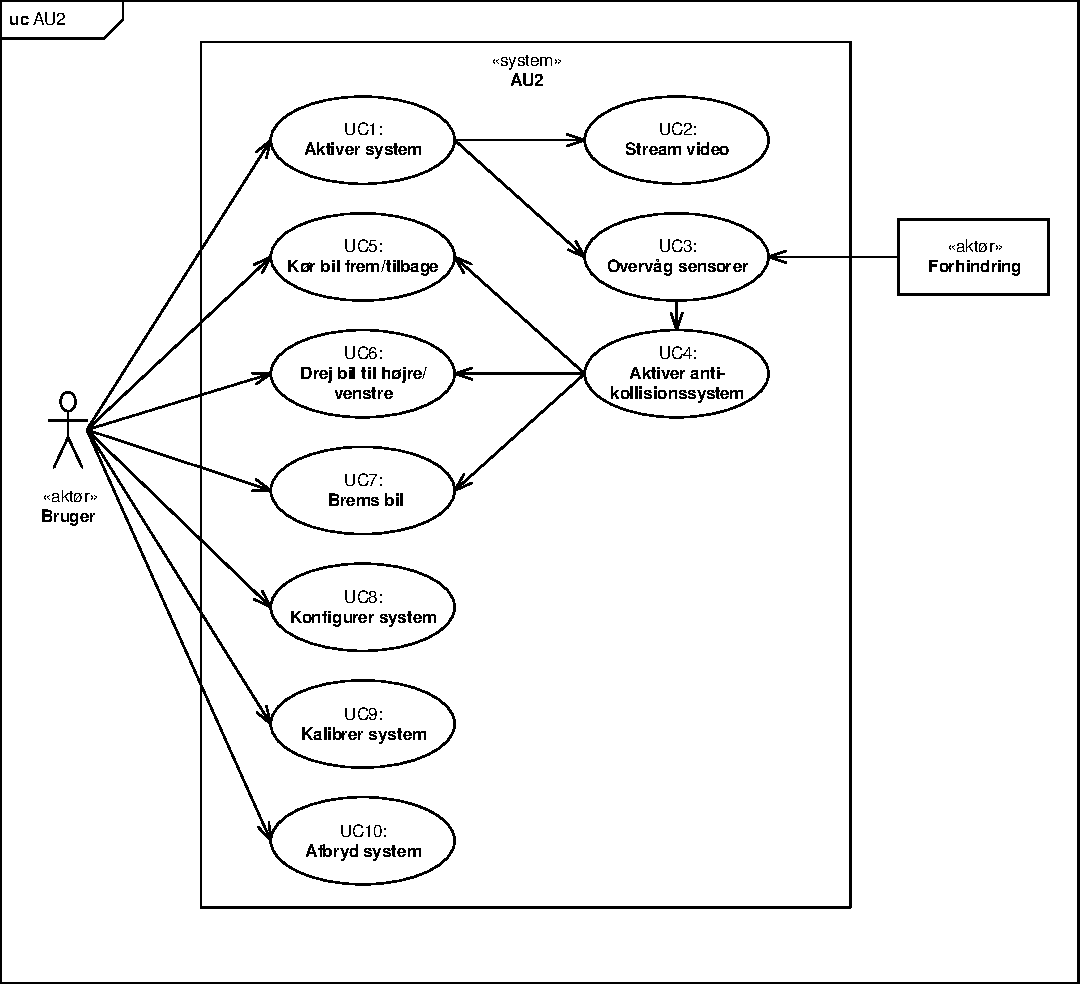
\includegraphics[width=\textwidth - 1 cm]{../fig/diagrammer/uc_au2.pdf}
\caption{Use case diagram for AU2.}
\label{fig:UC_au2}
\end{figure}
\clearpage

%----------------------------------------------------------------------------------------
%								Use Case beskrivelser - Initiering og Formål
%----------------------------------------------------------------------------------------

\subsection{Use Case beskrivelser - Initiering og Formål} 
\subsubsection{UC1: Aktiver system}
Initieres af: Bruger

Denne UC giver Bruger mulighed for at aktivere systemet. Bruger åbner software på PC, og sætter bilens ''ON/OFF''-knap til ''ON'' for at tilslutte batteriet. Herefter konfigureres bilen, UC2 + UC3 initieres og PC'en viser hovedvinduet. 

\subsubsection{UC2: Stream Video}
Initieres af: UC1: Aktiver system

Denne UC initierer videostream fra kameraet, og forbindelsen over Wi-Fi netværket oprettes.

\subsubsection{UC3: Overvåg sensorer}
Initieres af: UC1: Aktiver system

Denne UC initierer overvågning af bilens sensorer, herunder, de 4 afstandssensorer, tachometer, samt accelerometer. Use casen kører kontinuerligt og henter løbende data fra sensorerne.

\subsubsection{UC4: Undvig forhindring}
Initieres af: UC3: Overvåg sensorer

Denne UC har til formål at lade AKS overtage styring af bilen under kørsel hvis en forhindring detekteres enten foran eller bagved bilen.
Når forhindringen er undveget overgives styringen igen til Bruger.

\subsubsection{UC5: Kør bil frem/tilbage}
Initieres af: Bruger

Denne UC har til formål at give Bruger mulighed for at ændre hastighed på bilen via  de trykfølsomme ''LT'' og ''RT''-knapper på Xbox-360 controlleren. Bruger trykker på ''LT'' og bilen kører fremad, eller Bruger trykker på ''RT'' og bilen bakker.

\subsubsection{UC6: Drej bil til højre/venstre}
Initieres af: Bruger

Denne UC har til formål at lade Bruger ændre bilens retning. Bruger benytter venstre styrepind på Xbox-360 controlleren. Føres styrepinden til venstre, drejer bilens forhjul til venstre. Føres styrepinden til højre, drejer bilens forhjul til højre. Det har ingen betydning hvis styrepinden samtidig føres lidt opad eller nedad.

\subsubsection{UC7: Brems bil}
Initieres af: Bruger

Denne UC har til formål at lade Bruger sænke bilens hastighed. Bruger trykker ''X'' på Xbox-360 controlleren, jo længere tid knappen holdes nede jo mere sænkes bilens hastighed. Deaccelerationen er konstant.

\subsubsection{UC8: Konfigurer IP-adresse}
Initieres af: Bruger

Denne UC har til formål at lade Bruger konfigurere PC'ens IP-adresse således at der kan opnås forbindelse til bilen.  

\subsubsection{UC9: Tænd/sluk AKS}
Initieres af: Bruger

Denne UC har til formål at give Bruger mulighed for at vælge om AKS skal være tændt eller slukket. Bruger kan via ''Hovedvindue'' på PC'en vælge status for AKS. 

\subsubsection{UC10: Indstil makshastighed}
Initieres af: Bruger

Denne UC har til formål at give Bruger mulighed for at indstille en maksimumhastighed på bilen. Hastigheden indstilles via PC'ens ''Hovedvindue''.

\subsubsection{UC11: Kalibrer styretøj}
Initieres af: Bruger

Denne UC har til formål at give Bruger mulighed for at kalibrere bilens styretøj, så den kører ligeud når styrepinden ikke påvirkes. Bruger indtaster via menuen ''Kalibrer styretøj'' en værdi der angiver center for styretøjet.

\subsubsection{UC12: Afbryd system}
Initieres af: Bruger

Denne UC har til formål at lade Bruger afbryde hele systemet. Bruger afslutter software på PC, og sætte bilen ''ON/OFF''-knap til ''OFF'' for at afbryde forbindelse til batteriet. 
\clearpage

%----------------------------------------------------------------------------------------
%									Use Case fully dressed
%----------------------------------------------------------------------------------------

\subsection{Fully Dressed Use Cases}

% UC1:  Aktiver system
\begin{longtable}{| l | >{\raggedright}X | >{\raggedright}X | >{\raggedright}X | >{\raggedright\arraybackslash}p{2.3cm} |} \hline
	\multicolumn{2}{|l|}{\textbf{Use case under test}} & 
	\multicolumn{3}{l|}{UC1: Aktiver system} \\ \hline
	
	\multicolumn{2}{|l|}{\textbf{Scenarie}} & 
	\multicolumn{3}{l|}{Hovedscenarie} \\ \hline
	
	\multicolumn{2}{|l|}{\textbf{Forudsætning}} & 
	\multicolumn{3}{p{10.2cm}|}{Netværksforbindelse er opsat og fungerende\hfill} \\ \hline
	%\multicolumn{5}{|l|}{}\\ \hline
	\textbf{Step} & \textbf{Handling} & \textbf{Forventet Resultat} & \textbf{Resultat} & \textbf{Godkendt / Kommentar} \\ \hline

	1.1 & Bruger sætter bilens ''ON/OFF''-switch til ''ON''. 
		& Visuel test:\\ Lampe på bilens strømforsyning lyser.
		& Lampen lyser ikke, strømforsyning kan høres. Pi og PSoC starter op og deres respektive LEDer lyser.
		& IKKE OK - Forsyning til lampe på strømforsyningen er ikke forbundet.\\ \hline
		
	1.2 & Bruger starter software på PC.
		& Visuel test:\\ Hovedvinduet vises på skærmen.
		& Hovedvinduet ses på skærmen
		& OK\\ \hline
		
	1.3 & Bruger trykker på ''Opret forbindelse''.
		& Visuel test:\\ Hovedvindue viser ''Forbindelse oprettet''.
		& En pop-op med forbindelse oprettet vises
		& OK\\ \hline
		
	1.4 & Bruger observerer hovedvinduet.
		& Visuel test:\\ Videostream vises i hovedvinduet.
		& Videostream kan ses i hovedvinduet
		& OK\\ \hline
		
	1.5 & Bruger observerer hovedvinduet.
		& Visuel test:\\ Bilens aktuelle hastighed vises i hovedvinduet.
		& Bilens hastighed vises i hovedvinduet, opdateres dog ikke hvis bilen står stille (viser ej 0 km/t)
		& OK\\ \hline
		
	1.6 & Bruger observerer hovedvinduet.
		& Visuel test:\\ Bilens aktuelle tyngdeacceleration vises i hovedvinduet.
		& Acceleration G opdateres ikke
		& IKKE OK - Accelerometer er ikke implementeret.\\ \hline
		
	1.7 & Bruger observerer hovedvinduet.
		& Visuel test:\\ Data fra bilens afstandssensorer vises i hovedvinduet.
		& Hovedvinduet viser korteste afstand for sensorerne i meter - ikke præcis over 1m
		& OK\\ \hline
		
\caption{Accepttest for UC1: Aktiver system}\label{tbl:acceptuc1}
\end{longtable}
\clearpage

% UC2: Stream Videofeed
\begin{longtable}{| l | >{\raggedright}X | >{\raggedright}X | >{\raggedright}X | >{\raggedright\arraybackslash}p{2.3cm} |} \hline
	\multicolumn{2}{|l|}{\textbf{Use case under test}} & 
	\multicolumn{3}{l|}{UC2: Stream Video} \\ \hline
	
	\multicolumn{2}{|l|}{\textbf{Scenarie}} & 
	\multicolumn{3}{l|}{Hovedscenarie} \\ \hline
	
	\multicolumn{2}{|l|}{\textbf{Forudsætning}} & 
	\multicolumn{3}{p{10.2cm}|}{UC1 frem til punkt 5 er fuldført \hfill} \\ \hline
	%\multicolumn{5}{|l|}{}\\ \hline
	\textbf{Step} & \textbf{Handling} & \textbf{Forventet Resultat} & \textbf{Resultat} & \textbf{Godkendt / Kommentar} \\ \hline

	2.1 & Bruger åbner AU2 softwaren på PC'en og trykker ''Opret forbindelse''. %TODO: Dobbelttjek navngivning her.
		& Visuel test:\\ Der vises et live-feed fra bilens kamera.
		& Videostream kan ses i hovedvinduet.
		& OK\\ \hline
	2.2 & Bruger har Wireshark åbent på samme computer. Wireshark er opsat til at overvåge det pågældene netværk.
		& Visuel test:\\ I Wireshark observeres der for overføring af pakker fra bilens IP-adresse til computerens IP-adresse.
		& Der overføres pakker fra Pi til computeren.
		& OK\\ \hline
		
\caption{Accepttest for UC2: Stream Video}\label{tbl:acceptuc2}
\end{longtable}
\clearpage

% UC3: Overvåg sensor
\subsubsection{Use Case 3: Overvåg sensor}

%-------------------- UC3 --------------------
\begin{table}[h]
\begin{tabularx}{\textwidth}{| >{\raggedright\arraybackslash}p{3.3 cm} | >{\raggedright\arraybackslash}X |} \hline

\textbf{Navn:} 						 & UC3: Overvåg sensorer				\\ \hline
\textbf{Mål:}						 & At overvåge sensorer 				\\ \hline
\textbf{Initiering:}				 & UC1: Aktiver system 					\\ \hline
\textbf{Aktører:} 					 & Ingen 								\\ \hline
\textbf{Reference:} 				 & UC1, UC4: Undvig forhindring,UC9: Tænd/sluk AKS	\\ \hline
\textbf{Antal samtidige forekomster:}& Én 									\\ \hline
\textbf{Forudsætning:} 				 & UC1 frem til punkt 7 er fuldført		\\ \hline
\textbf{Resultat:}					 & Sensorer overvåges løbende  			\\ \hline
\textbf{Hovedscenarie:}				 & 

\begin{packed_enum}
	\item Bilen initierer tachometer
		\begin{packed_item}\itemsep1pt \parskip0pt \parsep0pt
			\item {[}Ext 1.a: Initiering af tachometer fejler{]}
		\end{packed_item}
	\item Bilen initierer accelerometer
		\begin{packed_item}\itemsep1pt \parskip0pt \parsep0pt
			\item {[}Ext 2.a: Initiering af accelerometer fejler{]}
		\end{packed_item}
	\item Bilen initierer afstandssensorer.
		\begin{packed_item}\itemsep1pt \parskip0pt \parsep0pt
			\item {[}Ext 3.a: Initiering af afstandssensorer fejler{]}
		\end{packed_item}
	\item Bilen overvåger sensorer.
	\item UC4: Undvig forhindring initieres af System
	\begin{packed_item}\itemsep1pt \parskip0pt \parsep0pt
			\item {[}Ext 5.a: AKS er slukket via UC9: Tænd/sluk AKS{]}
		\end{packed_item}
	\item Bilen modtager data fra PC.
	\item Bilen sender sensor data til PC.
\end{packed_enum} 															\\ \hline

\textbf{Udvidelser:}				&  
\textbf{{[}Ext 1.a : Initiering af tachometer fejler{]}}
	\begin{packed_enum}\itemsep1pt \parskip0pt \parsep0pt
		\item Systemet prompter PC med ''tachometer-initiering fejlet''.
		\item UC2 afsluttes.
	\end{packed_enum}	
														
\textbf{{[}Ext 2.a : Initiering af accelerometer fejler{]}}
	\begin{packed_enum}\itemsep1pt \parskip0pt \parsep0pt
		\item Systemet prompter PC med ''accelerometer-initiering fejlet''.
		\item UC2 afsluttes.
	\end{packed_enum}
	
\textbf{{[}Ext 3.a : Initiering af afstandssensorer fejler{]}}
	\begin{packed_enum}\itemsep1pt \parskip0pt \parsep0pt
		\item Systemet prompter PC med ''afstandssensor-initiering fejlet''.
		\item UC2 afsluttes.
	\end{packed_enum}
	
	\textbf{{[}Ext 5.a : AKS er slukket via UC9: Tænd/sluk AKS{]}}
	\begin{packed_enum}\itemsep1pt \parskip0pt \parsep0pt
		\item Use casen fortsætter fra punkt 6.
	\end{packed_enum}														\\\hline

\end{tabularx}
\caption{UC3: Overvåg sensorer}
\label{tbl:UC3}
\end{table}
\clearpage

% UC4: Anvend AKS

\begin{longtable}{| l | >{\raggedright}X | >{\raggedright}X | >{\raggedright}X | >{\raggedright\arraybackslash}p{2.3cm} |} \hline
	\multicolumn{2}{|l|}{\textbf{Use case under test}} & \multicolumn{3}{l|}{UC4: Undvig forhindring} \\ \hline
	\multicolumn{2}{|l|}{\textbf{Scenarie}} & \multicolumn{3}{l|}{Hovedscenarie} \\ \hline
	\multicolumn{2}{|l|}{\textbf{Forudsætning}} & \multicolumn{3}{p{10.2cm}|}{UC1 er gennemført, UC3 er gennemført.\hfill} \\ \hline
	%\multicolumn{5}{|l|}{}\\ \hline
	\textbf{Step} & \textbf{Handling} & \textbf{Forventet Resultat} & \textbf{Resultat} & \textbf{Godkendt / Kommentar} \\ \hline
	
	4.1 & Bruger styrer bilen fremad mod en forhindring på min. $(30cm \times 30cm)$ vinkelret på bilens kørebane vha. Xbox-360 controlleren, således at bilen er umiddelbart til venstre for objektet. & Visuel test: \\ Bruger observerer at bilen ændrer kurs til højre på trods af brugerinput. & ~ & ~ \\ \hline
	
	4.2 & Bruger tester om det er muligt at styre bilen igen med Xbox-360 controlleren. & Visuel test: \\ Bruger observerer at bilen reagerer på brugerinput. & ~  & ~ \\ \hline
	
	4.3 & Bruger styrer bilen fremad mod en forhindring på $(30cm \times 30cm)$ vinkelret på bilens kørebane vha. Xbox-360 controlleren, således at bilen er umiddelbart til højre for objektet. & Visuel test: \\ Bruger observerer at bilen ændrer kurs til venstre på trods af brugerinput. & ~ & ~\\ \hline
	
	4.4 & Bruger styrer bilen fremad mod en forhindring på $(30cm \times 30cm)$ vinkelret på bilens kørebane vha. Xbox-360 controlleren, således at bilen har retning lige mod objektet. & Visuel test: \\ Bruger observerer at bilen standser på trods af brugerinput. & ~ & ~ \\\hline
	
	4.5 & Bruger bakker mod en forhindring på $(30cm \times 30cm)$ vinkelret på bilens kørebane vha. Xbox-360 controlleren, således at bilen er umiddelbart til venstre for objektet. & Visuel test: \\ Bruger observerer at bilen ændrer kurs til venstre på trods af brugerinput. & ~ & ~ \\ \hline
	
	4.6 & Bruger bakker bilen mod en forhindring på $(30cm \times 30cm)$ vinkelret på bilens kørebane vha. Xbox-360 controlleren, således at bilen er umiddelbart til højre for objektet. & Visuel test: \\ Bruger observerer at bilen ændrer kurs til højre på trods af brugerinput. & ~ & ~\\ \hline
	
	4.7 & Bruger bakker bilen mod en forhindring på $(30cm \times 30cm)$ vinkelret på bilens kørebane vha. Xbox-360 controlleren, således at bilen har retning lige mod objektet. & Visuel test: \\ Bruger observerer at bilen standser på trods af brugerinput. & ~ & ~\\\hline

\caption{Accepttest for UC4: Undvig forhindring}\label{tbl:acceptuc4}
\end{longtable}
\clearpage

% UC5: Kør bil frem/tilbage
\subsection{Use Case 5: Kør bil frem/tilbage}
\begin{table}[h]
\begin{tabularx}{\textwidth}{| L{3.3 cm} | Z |} \hline

\textbf{Navn:} 						& UC5: Kør bil frem/tilbage\\ \hline
\textbf{Mål:}						& At få bilen til at køre frem eller tilbage. \\ \hline
\textbf{Initiering:}				& Bruger \\ \hline
\textbf{Aktører:} 					& Bruger \\ \hline
\textbf{Reference:} 				& Ingen \\ \hline
\textbf{Antal samtidige forekomster:} & Én \\ \hline
\textbf{Forudsætning:} 				& UC1: Aktiver system er fuldført og systemet er operationelt. \\ \hline
\textbf{Resultat:}					& Bilens hastighed er ændret. \\ \hline
\textbf{Hovedscenarie:}				& 

\begin{packed_enum}
\item Bruger ændrer position af RT på HID controlleren.
	\begin{packed_item}\itemsep1pt \parskip0pt \parsep0pt
	\item {[}Ext 1.a: Bruger ændrer position af LT.{]}
	\end{packed_item}
\item Controllerens input streames til bilen.
\item Bilen ændrer fremadgående hastighed i henhold til brugerens input. Et hårdere tryk resulterer i en højere hastighed og et lettere tryk resulterer i en lavere hastighed.
\item UC5 afsluttes.
\end{packed_enum} \\ \hline
\textbf{Udvidelser:}				&  
\textbf{{[}Ext 1.a : Bruger ændrer position af LT.{]}}
	\begin{packed_enum}\itemsep1pt \parskip0pt \parsep0pt
		\item Controllerens input streames til bilen.
		\item Bilen ændrer bagudgående hastighed i henhold til brugerens input. Et hårdere tryk resulterer i en højere hastighed og et lettere tryk resulterer i en lavere hastighed.
		\item Systemet fortsætter fra punkt 4 i hovedscenariet.
	\end{packed_enum}
\\ \hline
\end{tabularx}
\caption{UC5: Kør bil frem/tilbage}
\label{tbl:UC5}
\end{table}
\clearpage

% UC6: Drej bil til højre/Venstre
\subsection{Use Case 6: Drej bil til højre/venstre}
\begin{table}[h]
\begin{tabularx}{\textwidth}{| L{3.3 cm} | Z |} \hline

\textbf{Navn:} 						& UC6: Drej til højre/venstre\\ \hline
\textbf{Mål:}						& At få bilen til at dreje mod højre eller venstre. \\ \hline
\textbf{Initiering:}				& Bruger \\ \hline
\textbf{Aktører:} 					& Bruger eller AKS \\ \hline
\textbf{Reference:} 				& Ingen\\ \hline
\textbf{Antal samtidige forekomster:} & Én \\ \hline
\textbf{Forudsætning:} 				& UC1: Aktiver system er fuldført og systemet er operationelt. \\ \hline
\textbf{Resultat:}					& Retningen på bilens forhjul er ændret. \\ \hline
\textbf{Hovedscenarie:}				& 

\begin{packed_enum}
\item Bruger ændrer position på den venstre styrepind på HID controlleren.
	\begin{packed_item}\itemsep1pt \parskip0pt \parsep0pt
	\item {[}Ext 1.a: AKS er aktiveret.{]}
	\end{packed_item}
\item Controllerens input streames til bilen.
\item Bilen tjekker input, hvis den er mere mod venstre drejer hjulet mere til venstre og omvendt. %TODO dette skal lige finpudses lidt.
\item UC6 afsluttes.
\end{packed_enum} \\ \hline
\textbf{Udvidelser:}				&  
\textbf{{[}Ext 1.a : AKS er aktiveret.{]}}
	\begin{packed_enum}\itemsep1pt \parskip0pt \parsep0pt
		\item Bilen analyserer input fra UC3.
		\item Bilen drejer til højre, hvis sensor FL registrerer en forhindrer, ditto venstre og FR.
		\item Bilen undviger forhindringen. %TODO Skal eventuelt lige finpudses
		\item Systemet fortsætter fra punkt 3 i hovedscenariet.
	\end{packed_enum}
\\ \hline
\end{tabularx}
\caption{UC6: Drej til højre/venstre}
\label{tbl:UC6}
\end{table}
\clearpage

% UC7: Brems bil
\begin{longtable}{| l | >{\raggedright}X | >{\raggedright}X | >{\raggedright}X | >{\raggedright\arraybackslash}p{2.3cm} |} \hline
	\multicolumn{2}{|l|}{\textbf{Use case under test}}  & \multicolumn{3}{l|}{UC7: Brems Bil} \\ \hline
	\multicolumn{2}{|l|}{\textbf{Scenarie}} 			& \multicolumn{3}{l|}{Hovedscenarie} \\ \hline
	\multicolumn{2}{|l|}{\textbf{Forudsætning}} 		& \multicolumn{3}{p{10.2cm}|}{UC1: Aktiver system er fuldført og systemet er operationelt.\hfill} \\ \hline
	%\multicolumn{5}{|l|}{}\\ \hline
	\textbf{Step} 	& \textbf{Handling} & \textbf{Forventet Resultat} & \textbf{Resultat} & \textbf{Godkendt / Kommentar} \\ \hline
	7.1 & Bruger trykker på ''X'' knappen på Xbox-360 controlleren. 
		& Visuel test: Bruger observerer at bilens hastighed sænkes. 
		&   
		&  \\ \hline
	
\\ \hline
\caption{Accepttest for UC7: Brems Bil }\label{tbl:acceptuc7}
\end{longtable}
\clearpage

% UC8: Konfigurer IP-adresse
\subsection{Use Case 8: Konfigurer IP-adresse}
%-------------------- UC8 --------------------
\begin{table}[h]
\begin{tabularx}{\textwidth}{| >{\raggedright\arraybackslash}p{3.3 cm} | >{\raggedright\arraybackslash}X |} \hline

\textbf{Navn:} 						& UC8: Konfigurer IP-adresse										\\ \hline
\textbf{Mål:}						& At konfigurere bilens IP-adresse til PC'en						\\ \hline
\textbf{Initering:}					& Bruger 															\\ \hline
\textbf{Aktører:} 					& Bruger															\\ \hline
\textbf{Reference:} 				& Ingen																\\ \hline
\textbf{Antal samtidige forekomster:} & Én 																\\ \hline
\textbf{Forudsætning:} 				& UC1: Aktiver system er udført til punkt 3, 
									  bilen og PC er på samme netværk,systemet viser ''Hovedvindue'' 
									  samt at systemet er operationelt									\\ \hline
\textbf{Resultat:}					& IP adressen på bilen er indstillet								\\ \hline
\textbf{Hovedscenarie:}				& 

\begin{packed_enum}
	\item Bruger trykker på ''Konfigurer IP''.
	\item Konfigurationssmenuen for IP-adressen vises, og der er mulighed for at indtaste en IP-adresse.
	\item Bruger indtaster bilens IP-adresse.
	\item Bruger trykker ''Gem'' og system viser ''Hovedvindue''.
	\item Bruger trykker på ''Opret forbindelse''.
	\item Menuen indikerer at der er forbindelse til bilen.
	\begin{packed_item}\itemsep1pt \parskip0pt \parsep0pt
		\item {[}Ext 6.a Menuen indikerer at der ikke er forbindelse til bilen{]}
	\end{packed_item}
	\item Bruger trykker på ''Tilbage''.
	\item Systemet viser ''Hovedvindue''.
\end{packed_enum}																						\\ \hline
\textbf{Udvidelser:}				&  
\textbf{[}Ext 6.a Menuen indikerer at der ikke er forbindelse til bilen{]}
	\begin{packed_enum}\itemsep1pt \parskip0pt \parsep0pt
	\item Bruger gentager fra punkt 2 i hovedscenarie. 
	\end{packed_enum}																					\\ \hline
\end{tabularx}
\caption{UC8: Konfigurer IP-adresse}
\label{tbl:UC8}
\end{table}
\clearpage

% UC9: Tænd/sluk AKS
\subsection{Use Case 9: Tænd/sluk AKS}
%-------------------- UC9 --------------------
\begin{table}[h]
\begin{tabularx}{\textwidth}{| L{3.3 cm} | Z |} \hline

\textbf{Navn:} 						& UC9: Tænd/sluk AKS \\ \hline
\textbf{Mål:}						& At tænde eller slukke for AKS på bilen \\ \hline
\textbf{Initering:}					& Bruger \\ \hline
\textbf{Aktører:} 					& Bruger (primær) \\ \hline  
\textbf{Reference:} 					& UC11: Kalibrer system\\ \hline
\textbf{Antal samtidige forekomster:} & Én \\ \hline
\textbf{Forudsætning:} 				& UC1: Aktiver system er udført, bilen og PC er på samme netværk, at systemet viser ''Hovedmenu'' samt at systemet er operationelt\\ \hline
\textbf{Resultat:}					&  \\ \hline
\textbf{Hovedscenarie:}				& 

\begin{packed_enum}
\item Bruger trykker på ''AKS'' 
\item Menuen for AKS kommer frem og der er mulighed for at tænde/slukke for AKS 
\item Menuen indikerer om der er tændt/slukket for AKS
\item Bruger trykker tænd/sluk efter ønske
\item Bilen tænder/slukker for AKS systemet efter brugerens ønske
\item Menuen indikerer nuværende status af AKS
\end{packed_enum} \\ \hline
\textbf{Udvidelser:}				&  
~
\\ \hline
\end{tabularx}
\caption{UC9: Tænd/sluk AKS}
\label{tbl:UC9}
\end{table}
\clearpage

% UC10: Indstil maks. hastighed
\begin{longtable}{| l | >{\raggedright}X | >{\raggedright}X | >{\raggedright}X | >{\raggedright\arraybackslash}p{2.3cm} |} \hline
	\multicolumn{2}{|l|}{\textbf{Use case under test}}  & \multicolumn{3}{l|}{UC10: Indstil makshastighed} \\ \hline
	\multicolumn{2}{|l|}{\textbf{Scenarie}} 			& \multicolumn{3}{l|}{Hovedscenarie} \\ \hline
	\multicolumn{2}{|l|}{\textbf{Forudsætning}} 		& \multicolumn{3}{p{10.2cm}|}{UC1: Aktiver system er udført, bilen og PC er på samme netværk, at systemet viser ''Hovedvindue'' samt at systemet er operationelt.\hfill} \\ \hline
	%\multicolumn{5}{|l|}{}\\ \hline
	\textbf{Step} 	& \textbf{Handling} & \textbf{Forventet Resultat} & \textbf{Resultat} & \textbf{Godkendt / Kommentar} \\ \hline
	
	10.1 & Bruger trykker på ''Indstil makshastighed''. 
		 & Visuel test: \\ Hovedvindue viser menu med mulighed for at indtaste makshastighed fra 1-10 km/t. 
		 & Vindue med mulighed for indstilling af max hastighed vises.
		 & OK\\ \hline
	10.2 & Menuen viser bilens nuværende makshastighed. 
		 & Den nuværende makshastighed vises.
		 & Den nuværende makshastighed vises til højre.
		 & OK\\ \hline
	10.3 & Bruger indtaster bilens ønskede makshastighed. 
		 & Menuen viser den ønskede makshastighed. 
		 & Der vises den nye makshastighed 
		 & OK\\ \hline
	10.4 & Bruger trykker på ''Ok''. 
		 & Systemet viser den nye makshastighed. 
		 & Systemet viser den indstillede makshastighed
		 & OK\\ \hline
	10.5 & Bruger holder ''RT'' inde på Xbox 360 controlleren.
		 & Bilen accelerer til den angivne maksimalhastighed.
		 & Bilen ændrer makshastighed ift. den indtastede, dette er dog ikke målt præcist
		 & MÅSKE OK\\ \hline
		 
\caption{Accepttest for UC10: Indstil makshastighed }\label{tbl:acceptuc10}
\end{longtable}
\clearpage

% UC11: Kalibrer styretøj
\subsection{Use Case 11: Kalibrer styretøj}
%-------------------- UC11 --------------------
\begin{table}[h]
\begin{tabularx}{\textwidth}{| >{\raggedright\arraybackslash}p{3.3 cm} | >{\raggedright\arraybackslash}X |} \hline

\textbf{Navn:} 						& UC11: Kalibrer styretøj												\\ \hline
\textbf{Mål:}						& At kalibrere systemet så bilen kører ligeud 
									  når brugeren slipper styrepinden på Xbox-360 controlleren 			\\ \hline
\textbf{Initering:}					& Bruger 																\\ \hline
\textbf{Aktører:} 					& Bruger																\\ \hline
\textbf{Reference:} 			    & Ingen																	\\ \hline
\textbf{Antal samtidige forekomster:} & Én 																	\\ \hline
\textbf{Forudsætning:} 				& UC1: Aktiver system er udført, bilen og PC er på samme netværk, 
									  at systemet viser ''Hovedmenu'', at systemet er operationelt 
									  samt bilen holder stille												\\ \hline
\textbf{Resultat:}					& Bilens styretøj er kalibreret 										\\ \hline
\textbf{Hovedscenarie:}				& 

\begin{packed_enum}
	\item Bruger vælger ''Kalibrer styretøj''.
	\item Systemet viser menu for Kalibrering med mulighed for indtastning af værdi mellem -50 og 50. %TODO dette tal skal evt. rettes
	\item Bruger indtaster værdi. 
	\begin{packed_item}\itemsep1pt \parskip0pt \parsep0pt
		\item {[}Ext 3.a : Bruger indtaster ugyldig værdi{]} %TODO mellemrum mellem bogstav og :? Husk at rette i alle UC
	\end{packed_item}
	\item Bruger trykker på ''Gem''.
	\item Systemet gemmer værdien på bilen.
	\item Forhjulene drejer en absolut værdi mod enten, højre eller venstre: positiv værdi oversætte til højre, og negativ værdi oversættes venstre.
	\item Systemet returnerer til ''Hovedvindue''
\end{packed_enum} 																							\\ \hline
\textbf{Udvidelser:}					&  
\textbf{[}Ext 3.a : Bruger indtaster en ugyldig værdi{]}
	\begin{packed_enum}\itemsep1pt \parskip0pt \parsep0pt
		\item Systemet prompter: ''Ugyldig værdi, indtast en gyldig værdi.''
		\item Systemet fortsætter fra punkt 2 i hovedscenariet.
	\end{packed_enum}																						\\ \hline
\end{tabularx}
\caption{UC11: Kalibrer styretøj}
\label{tbl:UC11}
\end{table}
\clearpage

% UC12: Afbryd system
\begin{longtable}{| l | >{\raggedright}X | >{\raggedright}X | >{\raggedright}X | >{\raggedright\arraybackslash}p{2.3cm} |} \hline
	\multicolumn{2}{|l|}{\textbf{Use case under test}} & 
	\multicolumn{3}{l|}{UC12: Afbryd system} \\ \hline
	
	\multicolumn{2}{|l|}{\textbf{Scenarie}} & 
	\multicolumn{3}{l|}{Hovedscenarie} \\ \hline
	
	\multicolumn{2}{|l|}{\textbf{Forudsætning}} & 
	\multicolumn{3}{p{10.2cm}|}{UC1: Aktiver system er fuldført, bilen holder stille og systemet er operationelt\hfill} \\ \hline
	%\multicolumn{5}{|l|}{}\\ \hline
	\textbf{Step} & \textbf{Handling} & \textbf{Forventet Resultat} & \textbf{Resultat} & \textbf{Godkendt / Kommentar} \\ \hline

	12.1 & Bruger lukker ned for softwaren på PC'en. 
		 & Visuel test:\\ Hovedvinduet forsvinder fra skærmen.
		 & 
		 & \\ \hline
		
	12.2 & Bruger skubber kontakten ''ON/OFF'' på undersiden af bilen til position ''OFF''
		 & Visuel test:\\ Lampe på strømforsyning slukker.
	 	 & 
		 & \\ \hline
		
\caption{Accepttest for UC12: Afbryd system}\label{tbl:acceptuc12}
\end{longtable}
\clearpage